\epigraph{\textit{"When it's a humid day, we don't fabricate cells"\\"But\dots  don't you fabricate them in a glovebox?"\\"Of course."}}

\myparagraph{Abstract} The experimental methods are described here in a very detailed way, mixed with comments and warnings to the reader, trying to underline the critical points spotted over my PhD. Needless saying, the critical points in fabricating a complex electronic device such as a perovskite solar cells are many and neither a proper description can assure reproducibility.

\section{Materials}

	All anhydrous and non-anhydrous solvents had a reagent grade purity; were purchased from Sigma-Aldrich and used without any additional treatment.

	\Acr{fai}, \acr{mabr} and \acr{mai} were either synthesized (see \cpageref{methods-MAI}) or bought from GreatCell Solar.

	\PbItwo (99~\%), \PbBrtwo (99.999~\%), \CsI (99.999~\%), \PbCltwo (98~\%), anhydrous chlorobenzene, anhydrous \gls{dmf}, and anhydrous \gls{dmso} were bought form Sigma-Aldrich and kept in a nitrogen-filled glovebox.

	Titanium(IV) isopropoxide (97~\%), acetylacetone, and \glsdesc{litfsi} (\gls{litfsi}) were bought from Sigma-Aldrich.

	4-tert-butylpyridine and hydroiodic acid (57~m/m\% in water) were bought from Sigma-Aldrich and kept in a fridge (the colour of both these reagents change with ageing when kept out of the fridge).

	\Spiro was bought from 1-Material and stored in a nitrogen-filled glovebox.

	Methylamine in methanol (40~w/w\%, \SI{\approx9.8}{\Molar}) was bought from Tokyo Chemical Industry.

	\Tae1, \tae3, and \tae4 molecules were used as received from Inés García-Benito, Agustín Molina-Ontoria and Nazario Martín (IMDEA, Madrid). The synthesis of \tae1 has been described in \authoryear{Cabau2015a} and \authoryear{Choi2015b}. The synthesis of \tae3 and \tae4 has been described in CITATION.

	Patterned \gls{fto} substrates with sheet resistance of \SI{7}{\ohm\per\sq} (TEC7) on \SI{2.2}{\mm} thick and \SI{14.8x14.8}{\mm} wide Pilkington glass were bought from Xinyan Technology Ltd.

	Patterned \gls{ito} substrates with sheet resistance of \SI{15}{\ohm\per\sq} on \SI{1.1}{\mm} thick and \SI{15x15}{\mm} wide glass were bought from Xinyan Technology Ltd.

	Dust free cloths Super Polx 1200A \SI{23x23}{\cm} were bought from Berkshire.

	\Gls{pedotpss} Clevios P VP.AI 4083 was bought from Heraeus.
	
\section{Equipments}

	\myparagraph{Organic residuals removal} UV/ozone treatment was performed with a T10X10/OES ultra-violet ozone cleaning system from UVOCS. Most common failure: insufficient gas extraction flow detected by differential pressure meter on the rear, it can be partially configured via a screw.

	\myparagraph{Spin coating in air} Spin coating depositions in the clean room were performed with a Laurell WS-400BZ-6NPP-LITE spin coater.

	\myparagraph{Muffle oven} Calcination was performed with a muffle oven Hobersal HD-230 controlled with a Fuji Electric PXR-4. Most common failure: users setting very badly the heating ramp.
	
	\myparagraph{Titanium hotplate} As an alternative to the muffle oven, calcination was performed with a titanium hotplate Harry Gestigkeit PZ 28-3TD. Most common failures: controller failure and heating resistance breaks in a point, it can be unmounted and replaced.

	\myparagraph{Glovebox} Perovskite deposition was performed in a nitrogen-filled glovebox MBraun UNILab.

	\myparagraph{Spin coating in inert atmosphere} Spin coating depositions in the nitrogen-filled glovebox were performed with a SPIN150 equipment (this model does not require a gas inlet, which would be troublesome in a glovebox) from SPS Europe where the transparent cap was removed from the lid for helping solvent vapours removal. The internal side of the deposition chamber was covered with aluminium foil and this foil replaced between an user and the next. Most common failure: exhaustion of the supposedly \SI{20}{\year} lasting non-volatile SRAM (integrated circuit BattRam DS1230Y-85+ DIP28, a perfect example of planned obsolescence).

	\myparagraph{Precision hotplate} Perovskite layers annealing were performed with a highly homogeneous hotplate JP Selecta Plactronic.

	\myparagraph{Profilometer} Thicknesses were measured furrowing layers with an hard object and measuring the elevation profile with an Ambios Tech. XP-1 profilometer.

	\myparagraph{Optical microscope} Optical microscopy images were acquired with a Leica S6 D microscope.
	
	\myparagraph{UV-Vis-NIR absorbance} Absorbance measurements were carried out on a Lambda 1050 PerkinElmer spectrophotometer equipped with a PhotoMultiplier Tube, \ch{InGaAs} and \ch{PbS} detectors system, double beam optics, double monochromator and \ch{D2} and \ch{W} light sources.
	
	\myparagraph{PhotoLuminescence spectroscopy} Fluorescence measurements were carried out on a Fluorolog Horiba Jobin Yvon spectrofluorimeter equipped with photomultiplier detector, double monochromator and	Xenon light source.

	\myparagraph{Time Resolved PhotoLuminescence} PhotoLuminescence lifetime measurements were carried out on a Edinburgh Instruments LifeSpec-II based on the \gls{tcspc} technique, equipped with a PhotoMultiplier Tube detector, double subtractive monochromator and picosecond pulsed diode lasers source.
	
	\myparagraph{Thermal evaporator} High vacuum thermal depositions were performed with a MBraun vacuum deposition chamber connected with a scroll pump in series to a turbo pump. The inorganic and metallic materials deposition was managed by a Inficom SQC310C (firmware version 6.44) while the organic material deposition was controlled in a manual fashion with a CreaPhys temperature control unit CU~103. The deposition speed was sensed via two oscillating quartz sensors whose calibration tooling was performed yearly. The evaporation chamber was embedded in a MBraun MB200B glovebox module controlled by a MBraun MB20G.

	\myparagraph{Devices holder} The devices holder is designed for holding 4 devices with 4 independent diodes each (the bottom contact is assumed to be in common, the top ones are isolated) and consists in an airtight container topped with a quartz window. It was designed and fabricated by Ikerlan. The holder has at least one gold tip for each diode's electrode, the contact is ensured by springs pushing the tips towards the devices. A printed circuit board connects the gold tips to a coaxial connector via two rotatory selectors which allows to select the needed diode.

	\myparagraph{Solar simulator}\label{solarsimulator}Illumination for current-voltage scans was provided by a Sun 2000 solar simulator (\SI{150}{\W}) bought from ABET Technologies. The proper filters of the lamp were set to simulate the AM 1.5G solar spectrum. The light intensity at the measurement position was measured via the short circuit current of a small photodiode calibrated with a certified (NREL) silicon photodiode and regulated to \SI{1000}{\W\per\m\squared}. Most common failure: lamp power supply.

	\myparagraph{Current-voltage scans} Current-voltage scans were performed with a Tektronix Keithley 2400 with firmware revision C30 programmable digital source meter connected to a computer via a GPIB-USB-HS adapter from National Instruments, connected to the solar simulator for the shutter control via a RS-232 (Keithley side) to coaxial (solar simulator side), and connected to the device to measure via a coaxial (devices side) to 2 banana plugs (Keithley side). Even if Keithley is a remarkable piece of hardware, I observed various times sparks in my devices when connecting them to the equipment, so I warmly suggest to manually set the Keithley in current measure mode with zero applied voltage, start the measure with the devices not connected and finally connect the devices.

	\myparagraph{White \gls{led} illumination} Background illumination for \acr{tpv}, \acr{tpc}, and \acr{ce} measurements was provided via a white light \gls{led} ring assembled in-house with \gls{led} from LUXEON Lumileds.

	\myparagraph{Pulsed illumination} Perturbation illumination for \acr{tpv} and \acr{tpc} measurements was provided by a nanosecond PTI GL-3300 nitrogen laser. The wavelength was selected using a dissolved molecular dye. The pulse intensity was attenuated with a semi-transparent glass for ensuring the small perturbation regime. The spark in the nitrogen laser emits a strong and unwanted electromagnetic pulse that can be received from all non-coaxial cables and from the samples holder, adding a transient noise to the oscilloscope measurement.

	\myparagraph{Oscilloscope} The voltage transients for \acr{tpv}, \acr{tpc}, and \acr{ce} measurements were registered with a Yokogawa DLM2052 oscilloscope connected to the device holder via coaxial cable and to the computer via an USB2 port (the transfer speed could be better if an Ethernet connection were used). For each registered transient, \SI{12500}{points} were saved (the maximum record length for this oscilloscope is \SI{125}{Mpoints} and the maximum sampling rate is \SI{2.5}{Gpoints\per\s}).

	\myparagraph{\Gls{sem}, \gls{esem} and \gls{esem}-\gls{edx} imaging} Superficial and cross section \gls{sem} images were acquired using a Jeol JSM-6400 microscope. Superficial and cross section \gls{esem} images were acquired at low voltage (20 keV) and low vacuum in a FEI Quanta 600 FEG microscope. The cut for cross section was performed mechanically: A small angle grinder (from Dremel) was used for furrowing a diagonal line on the substrate glass side (opposite to the \gls{fto}), then using two pliers the substrate was forced as if it was to bend the glass and opening further the furrow.

%FT-IR ATR
%CycloVoltammetry CH instruments electrochemical workstation CHI660C
%IPCE
%red and blue LEDs
%TAS
%TEM
%raman
%xrd

\section{Synthesis, handling and purification}

	\subsection{\Acr{mai} synthesis}\label{methods-MAI}

		%Reference in laboratory notebook: [ig15, ig18, ig31, ig83].

		The synthetic method was inspired by \cite{Im2011a, Aharon2014, Williams2014, Etgar2012a, Nagaoka2015}.

		In a \SI{500}{\ml} one-necked flask (a big vessel helps later for drying) opened at air, \SI{14}{\ml} of a methylamine in methanol (40~w/w\%, \SI{\approx9.8}{\Molar}) were introduced. Dropwise, \SI{15}{\ml} of hydroiodic acid in water (57~m/m\%) was added while stirring and cooling at \SI{0}{\celsius}. This mixture was left stirring at room temperature and then still overnight covering the flask neck without completely closing it.
		The solution was evaporated in a vacuum-assisted rotatory evaporator at \SI{60}{\celsius}.
		The obtained white solid was scraped and transferred on a funnel with membrane filter (Sartorius, \gls{ptfe}). It was washed with diethyl ether and the diethyl ether discarded. The solid was dissolved with ethanol, using as little volume as possible and vacuum was used for forcing the ethanol through the filter. The solid was recrystallized pouring abundant diethyl ether, then filtered, washed with diethyl ether and dried at vacuum overnight.

	\subsection{Lead salts handling}

		Lead iodide and bromide bottles have to be opened in a nitrogen-filled glovebox. The failure in keeping the lead containing precursors away from oxygen seems to cause the formation of some lead oxide, a remaining non-soluble solid in the precursors solution which would have to be filtered away.

	\subsection{Dense titania precursors solution}\label{precursors_tio2}

		The precursor solution for the dense \TiOtwo layer was prepared using \SI{0.65}{\ml} of titanium(IV) isopropoxide and \SI{0.38}{\ml} of acetylacetone (strongly exothermic, add dropwise) in \SI{5}{\ml} of ethanol. The solution can be used just for a few days after preparation. Some hydrolysed product can be present in the solution, so it has to be filtered (\gls{ptfe}, \SI{0.2}{\um}) just before the usage. The reader should consider the more stable and commercial precursor titanium diisopropoxide bis(acetylacetonate) as a convenient alternative.

	\subsection{\Acr{mapicl} perovskite precursors solution}\label{precursors_mapicl}

		The solution was prepared in the laboratory.

		In a vial, \SI{400}{\mg} of \acr{mai} and \SI{230}{\mg} of \PbCltwo (98~\%) were weighted. Then \SI{1}{\ml} of anhydrous \gls{dmf} was added and the solution was stirred at \SI{65}{\celsius} for \SI{1.5}{\hour}. The solution was not filtered and was used the same day of preparation.

	\subsection{\Acr{csfamapbibr} perovskite precursors solution}\label{precursors_csfamapbibr}

		In a nitrogen-filled glovebox, \SI{507}{\mg} of \PbItwo, \SI{73.4}{\mg} of \PbBrtwo, \SI{172}{\mg} of \acr{fai} and \SI{22.4}{\mg} of \acr{mabr} were weighted and mixed in a \SI{5}{\ml} vial. For reducing the effect of static charging on the weighting process in the glovebox, a stainless steel weighing boat was specifically fabricated. Already at this phase some reactivity can be seen between the mixed solids (lead based perovskites are known to be possible to synthesize in a mechanosynthesis solid-solid fashion), nevertheless this mixture can be stored in the glovebox for weeks without any effect on the devices' resulting efficiency.

		The very day of the deposition, \SI{0.2}{\ml} of anhydrous \gls{dmso} and \SI{0.8}{\ml} of anhydrous \gls{dmf} were added to the solid mixture of precursors. The solution was vigorously stirred (a magnetic stirrer as big as the vial bottom allowed us to dissolve all the solid grains) at \gls{rt} for \SI{1}{\hour}. Heating or storing the solution for days has been observed to result in a yellow perovskite layer when deposited and annealed, so some kind of detrimental transformation is evident to happen in the solution, hindering its storage for long time. Finally \SI{42}{\ml} of
		a \SI{1.5}{\Molar} \CsI solution in \gls{dmso} were added to the previous solution. The solution was filtered (\gls{ptfe}, \SI{0.2}{\um}) just before its usage: Even if the solution looks clear it can contain solid particles.

	\subsection{\Spiro and other \gls{htm} solutions for bottom cathode cells}

		A solvent with additives mix was prepared adding \SI{197}{\umol} of 4-tert-butylpyridine (\SI{28.8}{\ul}) to \SI{1}{\ml} of anhydrous chlorobenzene, then \SI{32}{\umol} of \gls{litfsi} (\SI{9.1}{\mg}) were added. The presence of 4-tert-butylpyridine enables the solubility of \gls{litfsi} in chlorobenzene.

		\Glsdesc{spiro} (\spiro) \gls{htm} solution was prepared dissolving \SI{59.0}{\umol} of \spiro (\SI{72.3}{\mg}) in \SI{1}{\ml} of the aforementioned solvent with additives mix.

		Other \gls{htm} solutions for bottom cathode cells were prepared dissolving either \SI{29.5}{\umol} of \glsdesc{tae1} (\tae1, \SI{36.6}{\mg}), \SI{19.7}{\umol} of \glsdesc{tae3} (\tae3, \SI{24.4}{\mg}), or \SI{9.83}{\umol} of \glsdesc{tae4} (\tae4, \SI{12.1}{\mg}) in \SI{1}{\ml} of solvent with additives further diluted with chlorobenzene in a 1:1, 1:2, 1:5 ratio respectively, in order to preserve the \gls{htm} to additives molar ratio of the \spiro solution (roughly \SI{3}{\eq} of 4-tert-butylpyridine and \SI{0.5}{eq} of \gls{litfsi}). The lower concentrations were used due to the lower solubility of these \gls{htm} as compared to \spiro one.

		The solutions were prepared in a nitrogen-filled glovebox in order to have control over the oxygen oxidation degree of the molecules.

\section{Perovskite Solar Cells}

	The "top" or "bottom" naming refers to the cell orientation during fabrication, so the "bottom" layer is the one closer to the glass substrate.

	\subsection{Top Cathode Perovskite Solar Cells}\label{methods_top}

		\myparagraph{Anode and \gls{htm} Substrate Preparation}
			% based on ig77
			This process was performed in a class 7 clean room.

			\Gls{ito} coated substrates were cleaned in an ultrasound bath with acetone for \SI{15}{\min}, isopropanol for \SI{15}{\min} and rubbed with a dust-free cloth. Finally, an UV/ozone treatment was performed for \SI{20}{\min}.
			\Gls{pedotpss} was filtered on \gls{pes} membrane (\SI{0.22}{\um})
			and deposited via spin coating (static dispensing, \SI{110}{\ul}) with a first step where the speeds regulates the thickness of the layer and a second step for removing the residual liquid accumulated at the substrate corners. The conditions are reported in \cref{pedotpss_thickness} and the thicknesses were obtained via absorbance of the film at \SI{2150}{\nm} (the absorption in the visible region is very weak) calibrated to the a very thick layer measured with the profilometer. A rough relation between the thickness $d$ and the spinning speed $f$ (with \SI{1000}{\rpm\per\s} acceleration) was found as $d = \frac{1820}{\sqrt{f}}$. Substrates were dried at \SI{110}{\celsius} for \SI{20}{\min} and stored in a nitrogen-filled glovebox for avoiding moisture absorption.

			\begin{table}%[h]
				\caption{\Gls{pedotpss} deposition conditions and resulting thickness}\label{pedotpss_thickness}
				\begin{center}
					\begin{tabular}{c c c | c c c | c}
						\multicolumn{3}{c|}{\nth{1} step} & \multicolumn{3}{c|}{\nth{2} step} & \multirow{2}{*}{thickness}                                                    \\
						acceleration                      & speed                             & time                       & acceleration    & speed     & time    &          \\
						\si{\rpm\per\s}                   & \si{\rpm}                         & \si{\s}                    & \si{\rpm\per\s} & \si{\rpm} & \si{\s} & \si{\nm} \\
						\hline
						\rule[0ex]{-4pt}{3ex}
						1000                              & 1000                              & 60                         & 2000            & 2000      & 3       & 65       \\
						1000                              & 1600                              & 60                         & 2000            & 2000      & 3       & 45       \\
						1000                              & 4500                              & 30                         & 500             & 3500      & 30      & 27       \\
					\end{tabular}
				\end{center}
			\end{table}

		\myparagraph{\Acr{mapicl} Perovskite One Step Fabrication}
			% ig71
			The deposition process was performed in a nitrogen-filled glovebox.

			The precursors solution (see \cpageref{precursors_mapicl}) was deposited via spin coating (\SI{80}{\ul}, static dispensing, loading time \SI{5}{\s}) with an acceleration of \SI{1000}{\rpm\per\s}, a speed of \SI{1900}{\s} for \SI{40}{\s}. The substrate was moved directly to a hotplate at \SI{100}{\celsius} and annealed for \SI{80}{\min}, resulting in a \SI{430}{\nm} thick perovskite layer. The film is colourless just after deposition, then it turns to brown, yellow and finally black on the hotplate.

		\myparagraph{\Acr{mapi} Perovskite Two Step Fabrication}
			% based on ig79
			This process was performed in a nitrogen-filled glovebox
			while constantly purging with a nitrogen flow for reducing the \gls{dmf} and \gls{dmso} vapours concentration.

			\SI{460}{\mg} of \PbItwo were dissolved in \SI{1}{\ml} of a 23:2~v/v blend of anhydrous \gls{dmf} and anhydrous \gls{dmso}. This solution was stirred at \SI{50}{\celsius} for \SI{1}{\hour}. \SI{50}{\mg} of \acr{mai} were dissolved in \SI{1}{\ml} of a 3:1~v/v blend of anhydrous isopropanol and ethanol. A \PbItwo layer was deposited from the unfiltered solution via spin coating (static dispensing, \SI{80}{\ul}, loading time \SI{5}{\s}) with accelerations and speeds reported in \cref{mapi_thickness}. After \SI{60}{\s} from the start of the spin coating, the \acr{mai} solution (\SI{100}{\ul}) was dynamically dispensed on the centre of the spinning substrate with a \SI{100}{\ul} micropipette keeping it tilted and depositing an uninterrupted stream. The substrate was then moved directly from the spin coater to an hotplate at \SI{100}{\celsius} and annealed for \SI{15}{\min}. The thicknesses reported in \cref{mapi_thickness} were measured using the profilometer.

			\begin{table}%[h]
				\caption{\Acr{mapi} deposition conditions and resulting thickness}\label{mapi_thickness}
				\begin{center}
					\begin{tabular}{c c c | c}
						acceleration    & speed     & time    & thickness \\
						\si{\rpm\per\s} & \si{\rpm} & \si{\s} & \si{\nm}  \\
						\hline
						\rule[0ex]{-4pt}{3ex}
						2000            & 2000      & 90      & 360       \\
						4000            & 4000      & 90      & 250       \\
						8000            & 7500      & 90      & 180       \\
					\end{tabular}
				\end{center}
			\end{table}

		\myparagraph{\Gls{etm} and Cathode Deposition}
			% based on ig75
			The solution was prepared in the clean room (weighting fullerene derivatives in a glovebox would be difficult due to electrostatic phenomena) and the deposition process was performed in a nitrogen-filled glovebox.

			\SI{30}{\mg} of \acr{pcbm70} were dissolved in \SI{1}{\ml} of anhydrous chlorobenzene and stirred at \gls{rt} for \SI{1}{\hour}. This solution was filtered (\gls{ptfe}, \SI{0.2}{\um}) and deposited in a nitrogen-filled glovebox via spin coating (static dispensing, \SI{80}{\ul}, loading time \SI{5}{\s}) with accelerations and speeds reported in \cref{pcbm_thickness}. The thickness was estimated by absorbance at \SI{378}{\nm} calibrating the highest point with a profilometer measurement. A rough relation between the thickness $d$ and the spin speed $f$ was found as $d = \frac{3930}{\sqrt{f}}$ when a concentration of \SI{30}{\mg\per\ml} in chlorobenzene was used.

			\Gls{ito} contact was cleaned on two edges using swabs slightly wet with chlorobenzene and then \gls{dmso} (the solvent vapours can damage the perovskite layer, that's why this process is done after \gls{htm} deposition).

			\begin{table}%[h]
				\caption{\Acr{pcbm70} deposition conditions and resulting thickness, with a concentration of \SI{30}{\mg\per\ml}}\label{pcbm_thickness}
				\begin{center}
					\begin{tabular}{c c c | c}
						acceleration    & speed     & time    & thickness \\
						\si{\rpm\per\s} & \si{\rpm} & \si{\s} & \si{\nm}  \\
						\hline
						\rule[0ex]{-4pt}{3ex}
						1100            & 1100      & 80      & 120       \\
						2000            & 2000      & 60      & 90        \\
						4000            & 4000      & 40      & 60        \\
						8000            & 7500      & 20      & 40        \\
					\end{tabular}
				\end{center}
			\end{table}

			Finally, \SI{120}{\nm} of silver were deposited by thermal evaporation in high vacuum (\SI{1E-9}{\bar}). This resulted in four independent \SI{0.09}{\cm\squared} diodes for each substrate.
\label{methods_top_end}
	\subsection{Bottom Cathode Perovskite Solar Cells}

		\myparagraph{Cathode and \gls{etm} substrate preparation}
			This process was performed in a class 7 clean room.

			Pre-patterned \SI{1.5 x 1.5}{\cm} \gls{fto} coated glasses were employed as substrate. An identification code was scratched on the glass side with a diamond tip pencil. The glass dust was removed with adhesive tape and rubbing with a dust free cloth. The substrates were cleaned with ultrasonication in water with Hellmanex soap, then in deionized water, and finally in isopropanol; dried rubbing with a dust free cloth and the organic residuals were removed with an UV/ozone treatment for \SI{20}{\min}.

			Dense (as opposed to mesoporous) \TiOtwo layer was deposited (static dispensing, \SI{80}{\ul}) from the solution described in \cpageref{precursors_tio2} by spin-coating at \SI{3000}{\rpm}, \SI{3000}{\rpm\per\s}, for \SI{60}{\s} (\SI{\approx 30}{\nm}) over the previously cleaned \gls{fto}. The substrates were placed in a glass Petri dish kept slightly open (this helps the removal of the burnt organic residuals and manages to reduce the entrance of dust) and inserted in a muffle oven. The sintering can also be performed placing the substrates on a titanium hotplate, but the amount of dust on the deposited layer is greater. Then the substrates were sintered at \SI{500}{\celsius} for \SI{30}{\minute} and cooled down slowly for not breaking the Petri dish. Subsequently the substrates were immersed in a filtered (\gls{pes}, \SI{0.22}{\um}) \SI{40}{\milli\Molar}
			\ch{TiCl4} solution in 9~\% \ch{HCl} in an oven at \SI{70}{\celsius} for \SI{20}{\min} (this process erode the titania layer, so it's important to not exceed in the duration), cleaned with water, with isopropanol and calcined as aforementioned at \SI{500}{\celsius} for \SI{30}{\min}.

			The usage of a thicker glass as compared to the one used for top cathode cells and the usage of \gls{fto} in place of \gls{ito} (\gls{fto} absorbs more in the infrared region and is way rougher) are needed for resisting the high temperature processing of the titania layers.

			%\myparagraph{\Acr{mapi} Perovskite Two Step Fabrication}	
			% ig87

		\myparagraph{\Acr{csfamapbibr} Perovskite One Step Fabrication}

			This process was performed in a nitrogen-filled glovebox
			while constantly purging with a nitrogen flow for reducing the \gls{dmf} and \gls{dmso} vapours concentration.

			Perovskite precursor solution (see \cpageref{precursors_csfamapbibr}) was filtered (\SI{0.2}{\um}, \gls{ptfe})
			and deposited by spin-coating (\SI{80}{\ul}, static dispensing, first step \SI{1000}{\rpm}, \SI{1000}{\rpm\per\s}, \SI{10}{\s};
			second step \SI{6000}{\rpm}, \SI{1000}{\rpm\per\s}, \SI{20}{\s}; fast crystallization was induced dynamically
			dispensing \SI{50}{\ul} of chlorobenzene on the spinning substrate \SI{5}{\s} before the end of the second
			step) obtaining a \SI{500}{\nm} thick perovskite layer.

			The substrates were immediately transferred from
			the spin coater to a hot plate and annealed at \SI{100}{\celsius} for \SI{60}{\minute}.

			After removing from the hotplate, the devices were stored in a glass Petri dish for protecting from dust deposition. It was left partially open to avoid accumulation of vapours from solvent residuals.

		\myparagraph{\Gls{htm} and Cathode Deposition}

			The \gls{htm} solutions (\spiro, \tae1, \tae3, or \tae4) were filtered (\SI{0.2}{\um}, \gls{ptfe}) just before usage and deposited by spin-coating in a nitrogen-filled glovebox
			onto the perovskite layer (\SI{60}{\ul}, static dispensing, \spiro at \SI{4000}{\rpm}, \SI{4000}{\rpm\per\s},
			for \SI{30}{\s}; \tae1 and \tae3 at \SI{2000}{\rpm}, \SI{2000}{\rpm\per\s}, for \SI{30}{\s}; \tae4 at \SI{1000}{\rpm}, \SI{2000}{\rpm\per\s},
			for \SI{45}{\s}) and similar \gls{htm} thicknesses were obtained (\SI{\approx 100}{\nm}).

			\Gls{fto} contact was cleaned on two edges mechanically removing the \gls{htm} and perovskite with a needle and then using swabs slightly wet with \gls{dmso} (the solvent vapours can damage the perovskite layer, that's why this process is done after \gls{htm} deposition and just for what's remaining after mechanical scratching most of the material).

			Unless otherwise specified, in order to increase the
			oxidative doping of the \gls{htm} in a more or less controlled way, the devices were kept \SI{1}{\hour} in dark in a dry air chamber.

			Finally, \SI{80}{\nm} of gold was deposited by thermal evaporation in an ultra-high vacuum chamber
			(\SI{1e-9}{\bar}, MBraun) using a shadow mask leading to 4 diodes for substrate each with an active area of
			\SI{9}{\mm\squared}.

	\subsection{Handling and Preservation}
		In case of bottom cathode cells, the oxidation of the HTM has been proven to improve the PCE. The oxidation can be induced via a dopant, for example FK 209 Co(III) TFSI salt\cite{Burschka2013}, or via oxygen exposure. The latter has to be performed in dark as a synergic light and oxygen contribution on the perovskite layer degradation has been reported CITATION. The oxygen can enter in direct contact with the perovskite layer due to permeability of the HTM; additionally, when a mesoporous ETM is used (e.g. titania) oxygen can diffuse rapidly through the partially infiltrated mesoporous structure. For this reason a cabinet has been modified adding of a constant dry air inlet and physically reducing the leaks of the opening door edges.

		\begin{figure}%[!hbtp]%
			\makebox[\textwidth][c]{
				\parbox{1.1\textwidth}{
					\centering
					\begin{subfigure}[b]{0.5\textwidth}
						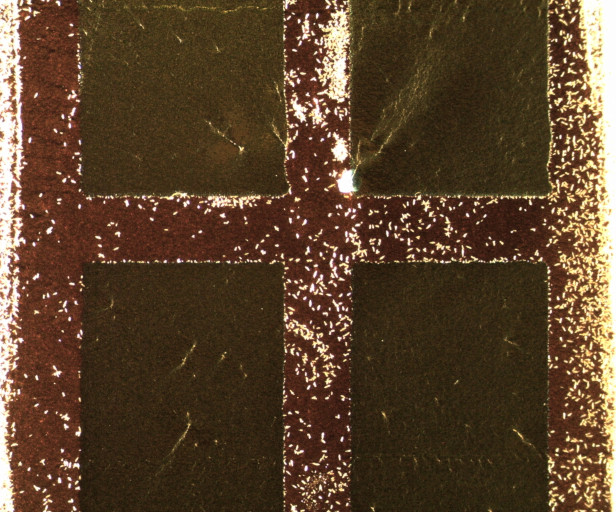
\includegraphics[width=1\textwidth]{microscope_degradation/ig93-1387-1-rescaled.jpg}
						\subcaption{Original cell, gold side.}\label{fig:microscope_degradation-start}
					\end{subfigure}
					\qquad
					\begin{subfigure}[b]{0.5\textwidth}
						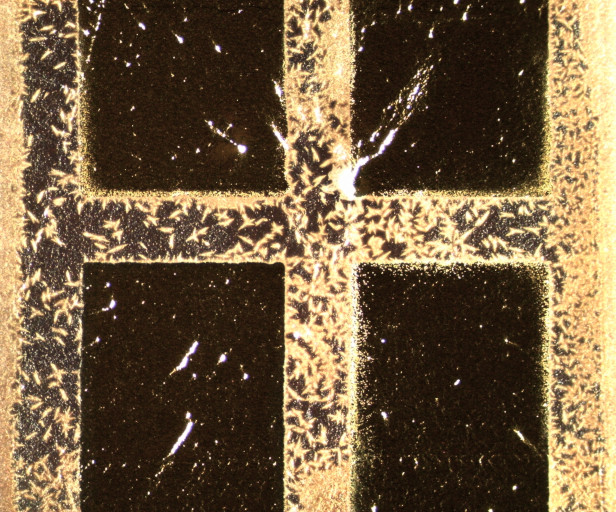
\includegraphics[width=1\textwidth]{microscope_degradation/ig93-1387-8-rescaled.jpg}
						\subcaption{After \SI{10}{\minute}, gold side.}\label{fig:microscope_degradation-end_front}
					\end{subfigure}
					\bigskip\newline

					\begin{subfigure}[b]{0.5\textwidth}
						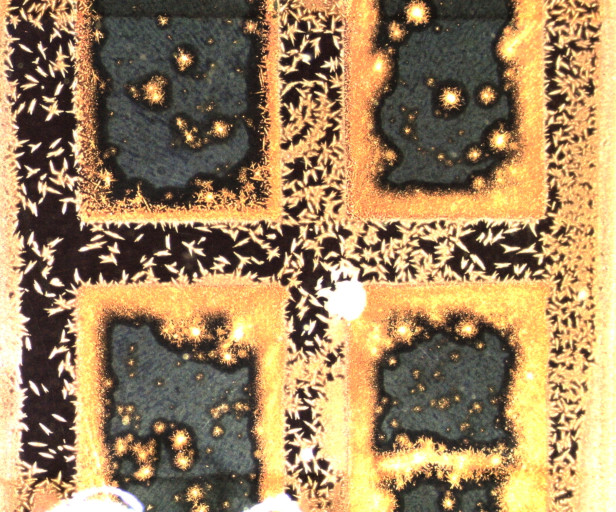
\includegraphics[width=1\textwidth]{microscope_degradation/ig93-1387-back-rescaled.jpg}
						\subcaption{After \SI{10}{\minute}, glass side.}\label{fig:microscope_degradation-end_back}
					\end{subfigure}
				}
			}
			\mycaption[Degradation due to oxygen and illumination combination.]{A \gls{fto}/\dTiOtwo/\mpTiOtwo/\acr{csfamapbibr}/\spiro/Au device upon \SI{10}{\minute} illumination in air.}\label{fig:microscope_degradation}
		\end{figure}

		In \cref{fig:microscope_degradation} the degradation of a complete device exposed to continuous illumination for 10 minutes and ambient air conditions is shown. An analogous device kept in air but without illumination did not show any degradation as observable via optical microscopy. The gold contact was not enough for protecting the perovskite layer from degradation, as oxygen could penetrate through the mesoporous titania. Interestingly the degradation is more prominent at metallic contacts' edges, one could speculate the reason being the electrical field being higher at smaller curvature metallic edges (seems that there's no therm in English for this, in Italian is referred as "effetto punta" and corona effect concentration ad edges derives from this). It could also be that the ionic profile of perovskite when holes quasi Fermi level is pinned at gold workfunction makes perovskite more sensible to degradation, and this is more evident at edges due to oxygen diffusion being blocked by the gold layer.

		Even if storage in dark and dry air should not be damaging for perovskite solar cells, usually the long-term storage happens in a nitrogen-filled glovebox.

\section{Solar Cells Characterization}

	All the characterization on complete devices was performed keeping them in a air tight holder filled with nitrogen. The electrical connection from the cell electrode to the external end of the holder was obtained via gold tips connected via a printed circuit board to a coaxial cable.
	
	\subsection{Sign Convention and Parameters Definitions}
	
	Considering a solar cell device at steady state under illumination and open circuit conditions, its cathode is defined as the contact where the electrons electrochemical potential $\bar\mu$ (Fermi level, the energy required for adding an electron, it depends mainly from the electrostatic potential $V$ and from the chemical potential $\mu$ due to the concentration of electrons) is the highest. By consequence the other contact is the anode. The naming of the two contacts holds to the one defined in illuminated, open circuit conditions even in conditions where the contacts' electrochemical potential is in the reversed order.
	
	The voltage $\Delta V$ is defined subtracting the electrons electrochemical potential of the cathode from the anode's one. So in the aforementioned conditions, the voltage is positive. The unit is the Volt.
	
	The electrical power $P$ is defined as positive when the device absorbs electrical energy (incoming, passive element) and negative when it generates energy (outgoing, active element). It can be expressed in extensive form with power (Watt) unit or in intensive form "electrical power density" with power (Watt) over active area (square centimetre) unit.
	
	The current $J=P/V$ is measured through an external circuit and the sign is a consequence of the voltage and electrical power definition: A current ("conventional current", flow of positively charged particles) being released from the device's anode and being received from the device's cathode is defined as negative. This can be thought as: Inside the device, somehow, a positive charge was moved from the high Fermi level contact to the low Fermi level contact, increasing its electrochemical energy, the opposite to what would happen in a resistor, whose current is always positive. In a solar cell device, the current and the electrical power can be either positive or negative depending on the illumination and voltage conditions. It can be expressed in extensive form with current (Amperes) unit or in intensive form "current density" with current (Amperes) per active area (square centimetre) unit.

		\Gls{voc} parameter is defined as the voltage $\Delta V$ at which the current is zero while the solar cell device is illuminated at 1~sun conditions and in steady state (positive by its own definition).

\Gls{jsc} parameter is defined as the unsigned value of the current density flowing in an external circuit short circuiting (zero resistance) the solar cell device's contacts while illuminated at 1~sun and in steady state. It is usually reported in current (milli Amperes) over active area (square centimetre) unit.

The maximum power is defined as the unsigned minimum of electrical power density which can be obtained by $P(V) = J(V) \cdot V$. It is usually reported using power (Watt) over active area (square centimetre) unit.

\Gls{pce} parameter is defined as the maximum power density over the illuminating power density, which at 1~sun AM 1.5G is defined to \SI{100}{\mW\per\square\cm}.

\Gls{ff} parameter is defined as the ratio between \gls{pce} and the product of \gls{voc} and \gls{jsc}. This parameter does not have a physical meaning, it just helps understanding how much factors like the series and the shunt resistance affect the device efficiency.

	\subsection{Shadowing Mask Was Not Used}
	
		In literature is generally suggested to use a shadowing mask when measuring the solar cell devices in order to better define the illuminated area (as in \cite{NatureResearch2017}, the file is an dynamic XFA form and cannot be opened by most PDF readers (and they rightly do not, as it was deprecated in ISO 32000-2:2017), Adobe products or Master PDF Editor is required for reading). In our case the active area is just \SI{0.09}{\square\cm} so the mask aperture should be extremely small and its exact positioning troublesome. Additionally, the fact that the illumination reaches the mask from a wide angle (the illuminating source dimension, which is not just the lamp as the illumination passes through spread lenses, is not small compared to the lamp-cell distance) allows the light to spread through the substrate glass (\SI{2.2}{\mm} for \gls{fto} substrates, other groups use even thicker glass substrates) reaching a significantly larger area on the active layer at the other side of the glass. In our solar simulator a linear widening of 8~\% over \SI{2}{\mm} was estimated, this makes an illuminated area 16~\% larger than the mask aperture. Even if the total incident power is still determined from the mask aperture, the illumination intensity is not 1~sun any more, compromising the validity of a measurement done with a shadowing mask.

	\subsection{Current-Voltage Sweeps}

		After calibrating the light intensity in the solar simulator (see \cpageref{solarsimulator}), the devices were exposed to the illumination at open circuit for some seconds in order to have a stabilized open circuit voltage. Then usually the curves were measured with the auto-measure function of the PyPV software (see \cpageref{automeasure}) which measures the reverse scan and then the forward scan.
		
		\myparagraph{Parameters Extraction from Sweeps}
			In the whole thesis, the reported values of \gls{voc}, \gls{jsc}, \gls{pce} and \gls{ff} are extracted from a forward or reverse current-voltage sweep. Checking the aforementioned definitions, one can easily notice how this is not the correct way as these parameters need to be measured in steady-state conditions. This is a widely accepted due to the tradition of solar cell reporting, which was established in pre-hysteresis times and is no longer a valid approximation. Apologizing for the lack of coherence I hope I'll be able to implement the static measurements of \gls{voc} and \gls{jsc} in the PyPV measurement routines (described in \cpageref{automeasure}). Regarding the \gls{pce}, and by consequence the \gls{ff}, a proper measurement is made difficult due to the cell evolution over time (hysteresis) which implies that the voltage associated to the maximum power point is drifting and the measurement affects this evolution. A proper \gls{mppt} system needs to be bought or developed, see \cpageref{software_mppt} for thoughts about possible implementations.

		\myparagraph{Scan speed}
			The used sweep speed is \SI{500}{\mV\per\s}, which was arbitrarily chosen for having an aesthetically good looking current-voltage curve (avoiding bumps leading to currents higher than \gls{jsc}), like the one in \cref{fig:iv_ugly}.

			\begin{SCfigure}%[!hbtp]%
				\centering
				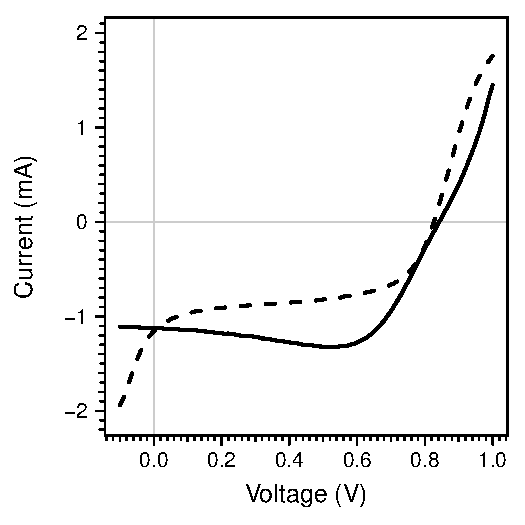
\includegraphics[width=0.5\textwidth]{iv_ugly/ig47-b32-int2-4.pdf}
				\mycaption[Hysteretic current-voltage scan.]{At the employed scan speed, the hysteresis phenomena causes the reverse (solid line) scan to reach currents higher than the \gls{jsc}.}\label{fig:iv_ugly}
			\end{SCfigure}

			Due to hysteresis phenomena, no scan speed, direction, or precondition is the correct one and they all heavily affect the resulting \gls{pce}. Indeed has been shown that even so-called "hysteresis-free" perovskite solar cells can have hysteresis on smaller or bigger time scale\cite{Jacobs2018}. Rather, a static measurement or a \acr{mppt} should be used for obtaining a result not completely alienated from the real world.

			The noise often observed in current-voltage scans at high sweep speeds is mainly caused by oscillations in the solar simulator illumination intensity, as an example see REFERENCE FIGURE. Indeed, using a white \gls{led} as illumination source, this noise is not present but the spectral mismatch affects the meaningfulness of the measurement.

		\myparagraph{Auto-scale}\label{autoscale}

			\begin{SCfigure}%[!hbtp]%
				\centering
				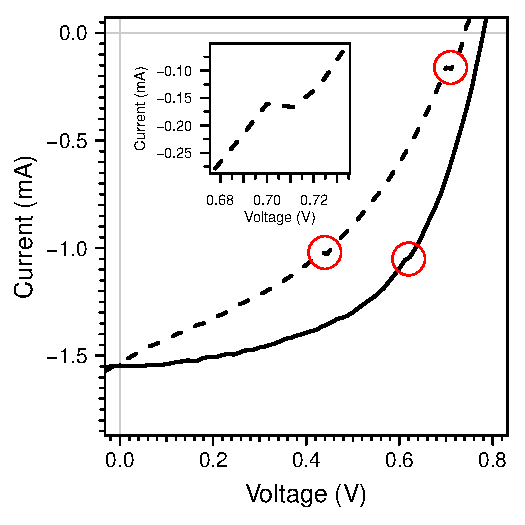
\includegraphics[width=0.5\textwidth]{autoscale/ig1-3-1-int4.pdf}
				\mycaption[Kinks in JV sweep due to autoscale.]{A current-voltage sweep of an hysteretic perovskite solar cell with Keithley autoscale active. Both the forward (dashed) and the reverse (solid line) present small discontinuities around \SI{1}{\mA} and \SI{0.1}{\mA}.}\label{fig:autoscale}
			\end{SCfigure}

			In literature one can easily find current-voltage curves with discontinuities and kinks\cite{Li2016,Snaith2014,Zhang2015} like the one reported in \cref{fig:autoscale}. Some even lucubrate about the origin of these in perovskite solar cells. Indeed this is likely just caused by the auto-scale feature of the Keithley equipment, disabling this, the discontinuities disappears.

	\subsection{\Gls{voc} and \gls{jsc} Dependence on Light Intensity}
		The illumination by solar simulation is reduced via neutral density filters with transmittance of 0.05, 0.12, 0.25, 0.51, 0.81 and 1 (no filter). The devices are kept at this reduced illumination $\phi$ and at open circuit or short circuit conditions until steady state for measuring respectively $V_{OC}(\phi)$ or $J_{SC}(\phi)$.
		
		\myparagraph{\Gls{jsc} versus $\bm{\phi}$}\label{methods_jsc_intensity} The \gls{jsc} dependency on the light intensity $\phi$ can be fitted with a power law $J_{SC} \propto \phi^\alpha$ giving $\alpha$ values usually from 0.95 to 1.
		
		\myparagraph{\Gls{voc} versus $\bm{\phi}$}\label{methods_voc_intensity} The \gls{voc} dependency on the light intensity $\phi$ can be fitted with a natural logarithmic (the base of the logarithm comes from Boltzmann distribution) dependence as:
		$$V_{OC} = k + \frac{n_{id} k_B T}{q}\cdot\ln(\phi)$$
		where $k$ does not contain physical meaning (depends on the light intensity units and on the \gls{voc} at 1~sun), $k_B$ is Boltzmann constant, $T$ is temperature in Kelvin, and $q$ is the elementary charge\cite{Calado2018b} (in literature one can found inexact reports of ideality factor determined via \gls{voc} versus \gls{jsc} dependency). The so-obtained ideality factor $n_{id}$ is usually from 1 to 2. In this thesis, this measurement is reported both from static measurement of \gls{voc} (proper method) and from \gls{voc} obtained from current-voltage sweeps; the used method is specified case by case.	An applied voltage dependent ideality factor can also be measured from a current-voltage sweeps in dark but has not been evaluated in this thesis. Anyway in perovskite solar cells exhibiting hysteresis, a current-voltage sweep would not give fair ideality factors and the current-voltage points should be acquired reaching steady state conditions for each point. Both these methods for deriving the ideality factor have been implemented in the DrIFtFUSION simulation as described in \cpageref{dd_ideality}.
		
		For the interpretation of these results, see \cpageref{interpretation_lightintensity}.
		
	\subsection{Charge Extraction (\acr{ce})}

		The device is kept under 1~sun equivalent illumination by a white \gls{led} at open circuit conditions until stabilization is reached. 1~sun equivalent illumination is defined as the illumination at which the a silicon photodiode gives the same \gls{jsc} as under calibrated 1~sun from the solar simulator. The \gls{led}-solar spectral mismatch affects slightly the measurement, but in no case a \gls{pce} is reported from any \gls{led}-illuminated experiment. After stabilization the illumination is switched off and, at the exactly same moment, the device is short circuited through a small and known resistance of \SI{50}{\ohm} \cite{Duffy2000}.

		This is repeated decreasing the light intensity from 1~sun down to dark (in dark no signal should be observed, indeed some residual charge can usually be seen, the reason of this could be ionic profile updating or an insufficient darkness) and a single decay is measured for each illumination point, over approximatively 30 illumination points.

		The equipment includes two transistors (in a in-house built circuit by Javier Pérez Hernández) connected to a pulse generator providing a square pulse long at least as the measurement window. I suggest to reduce as much as possible the duration of the dark period (ruled by the pulse generator) in order to save time for the stabilization step in the next measure.

		The measurement is carried out with an oscilloscope in parallel to the known small resistance. In the first microseconds, most of the free charge flows through the resistor generating a voltage drop across it which is measured by the oscilloscope. This potential drop can be converted to current using the Ohm's law, which, integrated over time, gives the amount of extracted charge.

		For the interpretation, see \cpageref{interpretation_ce}; for the implementation, see \cpageref{r_ce}.

		\myparagraph{Noise reduction}\label{r_ce_noise}
			Most of the observed short-times noise (\SI{< 5E-7}{\s}) is, supposedly, related to the opening and closing of the transistors included in the in-house built circuit.

			Annoyingly, the noise profile is characteristic of the cell and of the circuitry, so a simple average over many decays does not help in cancelling it.

			This affects the resulting measurement to a noticeable extent, which starts to be a problem if the charge versus light bias (\gls{voc} generated at a given illumination intensity) profile has to be studied in detail, as in \cref{ch:tae}.

			In order to reduce this effect various approaches have been tested; finally the single decays were fitted with a bi-exponential formula (sum of two exponential) and the integral of this fit was used.

	\subsection{Transient PhotoVoltage (\acr{tpv})}

		The device is kept under 1~sun illumination by a white \gls{led} ring at open circuit until stabilization is reached. 1~sun equivalent illumination is defined as the illumination at which the a silicon photodiode gives the same \gls{jsc} as under calibrated 1~sun from the solar simulator. Then an additional illumination pulse is provided by a nitrogen laser. The pulse duration is around \SI{1.5}{\ns}. The equipment can output up to 20~pulses per second, but due to the oscilloscope settings and oscilloscope internal memory speed we're limited to 1~pulse per second (maybe decreasing the number of acquired points would allow us to acquire higher repetition rates). The pulse was triggered with a square wave pulse generator. The wavelength is selected with the absorption and emission of a dissolved molecular dye, usually a wavelength of \SI{650}{\nm} is selected using a RhodamineB solution\cite{RadiantDyesLaser}, this wavelength allow us to illuminate in deep the perovskite layer (in contrast to a blue light where the illumination would be absorbed within the first hundreds of nanometres of the material).

		During all the process, the device is connected to a \SI{1}{\Mohm} oscilloscope, registering the open circuit voltage profile (the high resistance of the oscilloscope is a good approximation of open circuit). An auxiliary output from the square wave pulse generator used for the pulse is used for the trigger of the oscilloscope.

		The intensity of the laser pulse is decreased using a variable neutral density filter (a partially reflecting wheel with different positions for different transmittivities) so that the voltage perturbation caused by the light pulse does not exceed \SI{10}{\mV} with 1~sun background illumination intensity. We consider this as a "small-enough" perturbation.

		This process is repeated decreasing the light intensity from 1~sun down to dark. Clearly, the pulse intensity which could be considered a "small-enough" perturbation at high background illumination is not so at lower ones and cannot be small at dark conditions. We \emph{do not} regulate the pulse intensity depending from the background illumination for being able to use this data also for \acr{dc} studies. The \acr{dc} does not intrinsically need the usage of a constant pulse intensity but it needs the measurement of a \acr{tpc} for each pulse intensity. The switch from \acr{tpv} to \acr{tpc} setups and back would be complex and time demanding with the current setup. Anyway quite all the information from the \acr{tpv} is obtained from the high background illumination intensity measurements.

		For each illumination intensity, the reported decay is the result of averaging around 30~transients. This manages to reduce the noise.

		For the interpretation, see \cpageref{interpretation_tpv}; for the implementation, see \cpageref{r_tpv}.


		\myparagraph{Noise treatment}\label{tpv_robust}
			Most of the observed noise (\SI{< 2E-7}{\s}) is due to the radiofrequency emitted by the spark in the nitrogen laser which gets absorbed by the circuitry of the samples holder acting as a receiving antenna (the connection cables are coaxial, so they don't absorb radiofrequency). On the contrary to what happens for \acr{ce}, the short times noise seems to not follow a constant pattern, so averaging the measurement over a few repetitions (usually 30) manages to reduce the noise.

			This noise can affect the exponential or bi-exponential fitting, for this reason a robust fitting routine has been used, which gives a lower weight to outlier points. An example can be seen in \cref{fig:tpv_robust}.
			
			\begin{figure}
				\centering
				\includegraphics[width=0.9\textwidth]{{tpv_robust/TPV_ig52-68-3_0.883897_V-monoexp}.pdf}
				\mycaption[Robust and normal fitting comparison.]{In grey the fitted points, in yellow the points not considered for the fitting, the solid black line is the \gls{loess}. The normal non-linear least squares fitting (in green) is affected by noise, outliers and characteristics not of interest by the model. The non-linear robust fitting (in brown) manages to reduce the weight of these points.}\label{fig:tpv_robust}
			\end{figure}
		

		\myparagraph{Voltage Increase Value}\label{tpv_deltaV}

			The value of the voltage increase due to the additional illumination is needed for \acr{dc} measurement.

			In the group this $\Delta V$ value was traditionally obtained subtracting the steady state \gls{voc} from the maximum voltage point in the measured transient. This is obviously heavily affected by the aforementioned noise when a short time window is used.

			The following alternatives were tested:
			\begin{itemize}
				\item The linear factor in an exponential fit was used, but it can fail if the decay does not have a simple exponential shape (often a bi-exponential, sum of two exponentials, is observed);
				\item The sum of the two linear factors in a bi-exponential fit, which could work but one have to carefully set boundary values to the fitting parameters for avoiding a fast exponential matching just some noise;
				\item The maximum value of a \gls{loess} local regression was used, but this underestimates the value, especially when the peak top are just few points (when the measurement time window is large);
				\item The average of the values registered starting from the maximum voltage point and during a specified time lapse.
			\end{itemize}

			This last option is the one currently in place. The average was performed over \SI{50}{ns} after the peak and this allowed us to get a reliable $\Delta V$ value.

	\subsection{Transient PhotoCurrent (\acr{tpc})}

		The device is kept under 1~sun illumination by a white \gls{led} ring at short circuited through a \SI{50}{\ohm} resistor until stabilization is reached. 1~sun equivalent illumination is defined as the illumination at which the a silicon photodiode gives the same \gls{jsc} as under calibrated 1~sun from the solar simulator. Then an additional illumination pulse is provided by a nitrogen laser.

		The signal is acquired by an oscilloscope in parallel to the \SI{50}{\ohm} resistor. This allows us to measure a potential drop across the resistor and the related current via Ohm's law. Subtracting the constant current due to the background illumination and integrating the transient over time gives the charge generated by the laser pulse.

		This process is repeated at 1~sun and at dark background illumination conditions.

		For each illumination intensity, the reported decay is the result of averaging around 30~transients. This manages to reduce the noise.
		
		For the interpretation, see \cpageref{interpretation_tpc}; for the implementation, see \cpageref{r_tpc}.

	\subsection{Differential Capacitance (\acr{dc})}

		This is a meta-measurement as it just combines the data from \acr{tpv} and \acr{tpc} without requiring any additional experiment\cite{Shuttle2008}, sometimes also referred to as "differential capacitance".

		As explained in \cpageref{interpretation_dc}, the electrical capacitance of a solar cell is not a constant (as in most of the commercial capacitors), indeed it depends on the applied voltage bias or light bias.

		The charge obtained with the \acr{tpc} (in case the dark and illuminated results were different, the third quartile of all \acr{tpc} measurements was used) is divided by an array of values obtained from \acr{tpv}, one for each illumination intensity. The needed value is the \gls{voc} increase due to the laser pulse, prior to the decay to steady state, for each illumination intensity (obtained as described in \cpageref{tpv_deltaV}).

		This allows us to estimate the capacitance of the solar cell device at open circuit with various illumination intensities.

		For the interpretation, see \cpageref{interpretation_tpc}; for the implementation, see \cpageref{r_tpc}.